\chapter{Manual de usuario}
\label{chap:manual_usuario}

La primera vez que iniciemos la aplicación, se nos pedirá permisos para el acceso a archivos del móvil. Estos permisos son necesarios para que la aplicación pueda leer los archivos multimedia de el dispositivo móvil.

Una vez aceptados los permisos, introduciremos los datos para acceder a nuestra implementación en Lynx.js y se nos pedirá que introduzcamos los datos de conexión al servidor (ip y puerto). Estos datos se pueden modificar en cualquier momento desde el menú de configuración, pero hasta que no se introduzcan correctamente, no se podrá acceder a la aplicación.

En cuanto introduzcamos los datos de acceso al servidor, podremos iniciar sesión. Para iniciar sesión la primera vez, tendremos que utilizar la cuenta con usuario \texttt{admin} y la contraseña \texttt{admin}. Una vez iniciada la sesión, se nos pedirá crear una nueva cuenta, eliminando así la cuenta de administrador.


\begin{figure}[h]
  \centering
  \begin{minipage}[t]{0.3\textwidth}
    \centering
    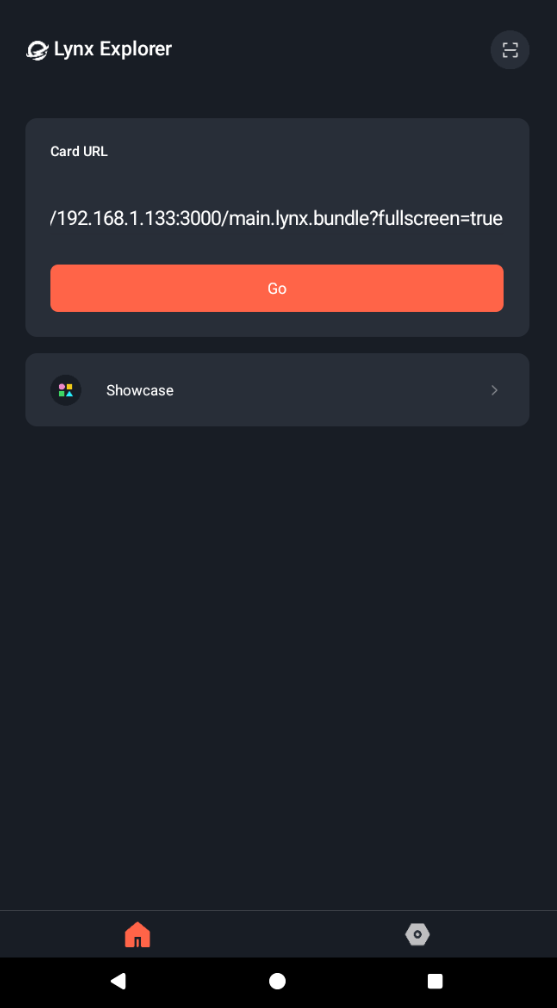
\includegraphics[width=\textwidth]{assets/lynx-application-url.png}
    \caption{Pantalla para introducir URL de la aplicación Lynx.js.}
    \label{fig:lynx-application-url}
  \end{minipage}
  \hfill
  \begin{minipage}[t]{0.3\textwidth}
    \centering
    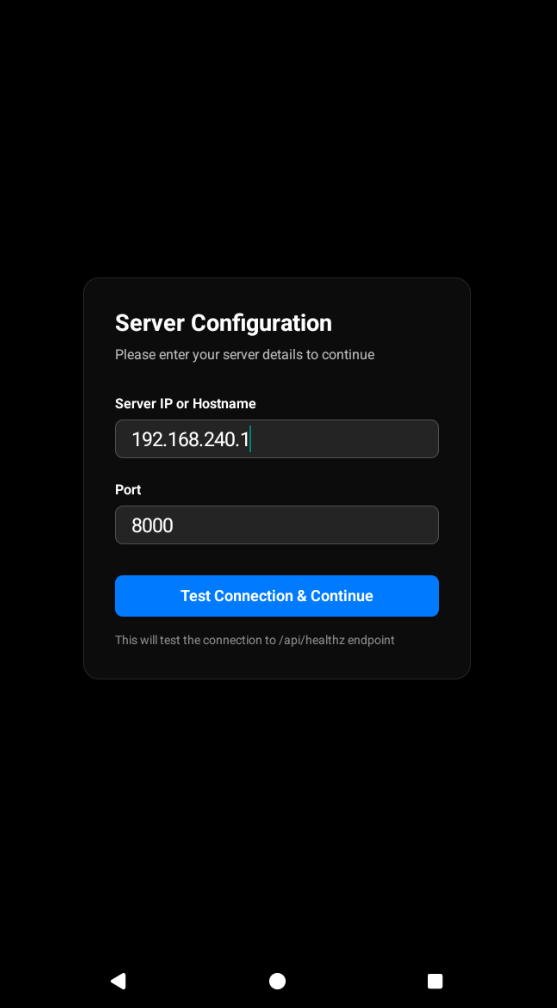
\includegraphics[width=\textwidth]{assets/server-settings-mobile.png}
    \caption{Pantalla de configuración del servidor en la aplicación móvil.}
    \label{fig:server-settings-mobile}
  \end{minipage}
  \hfill
  \begin{minipage}[t]{0.3\textwidth}
    \centering
    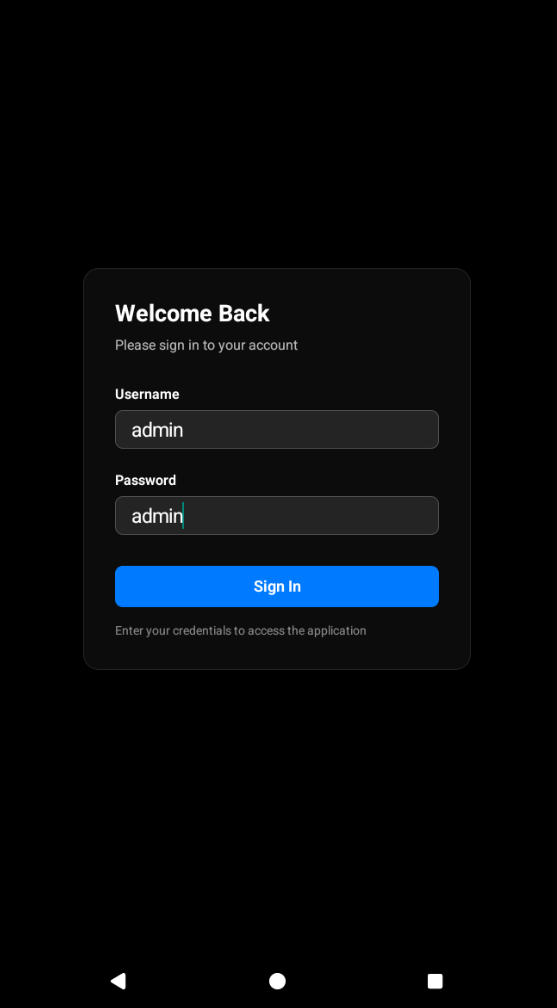
\includegraphics[width=\textwidth]{assets/login-screen-mobile.png}
    \caption{Pantalla de inicio de sesión en la aplicación móvil.}
    \label{fig:login-screen-mobile}
  \end{minipage}
\end{figure}

Al iniciar sesión, accederemos a la pantalla principal de la aplicación, donde podremos ver todos nuestros archivos multimedia del dispositivo, ordenados de más recientes a más antiguos.
Nos encontraremos con un menú de navegación en la parte inferior de la pantalla, donde podremos acceder a las diferentes secciones de la aplicación: Galería local, Galería online y Ajustes.

\section{Galería local}

Dentro de la galería local, disponemos de un botón de refresco en la parte superior derecha, que nos permitirá actualizar la lista de archivos multimedia en caso de que hayamos añadido o eliminado archivos desde fuera de la aplicación o queramos refrescar el estado de las mismas en el servidor. Contamos también con un botón que nos permitirá saber el estado del servidor en todo momento. Se comprueba si el servidor está activo cada 30 segundos, aunque se puede comprobar manualmente en cualquier momento tocando el botón que muestra el estado del servidor.

Desde nuestra galería local, podremos ver los archivos multimedia que tenemos en nuestro dispositivo con un distintivo para aquellos que ya han sido subidos al servidor. Si damos un toque a alguna imagen, abriremos una vista de detalle de la imagen, donde podremos ver la imagen en grande y subirla al servidor si no ha sido subida ya. En caso de que la imagen ya haya sido subida, podremos eliminarla del servidor.

Si mantenemos pulsada una imagen, podremos seleccionar varias imágenes a la vez para subirlas o eliminarlas del servidor. En la parte superior de la pantalla, aparecerá un menú contextual con las opciones disponibles para las imágenes seleccionadas.

Si el ajuste de sincronización automática está activado, al entrar en la galería local las imágenes se subirán automáticamente al servidor si no han sido subidas ya.

\begin{figure}[H]
  \begin{minipage}[t]{0.3\textwidth}
    \centering
    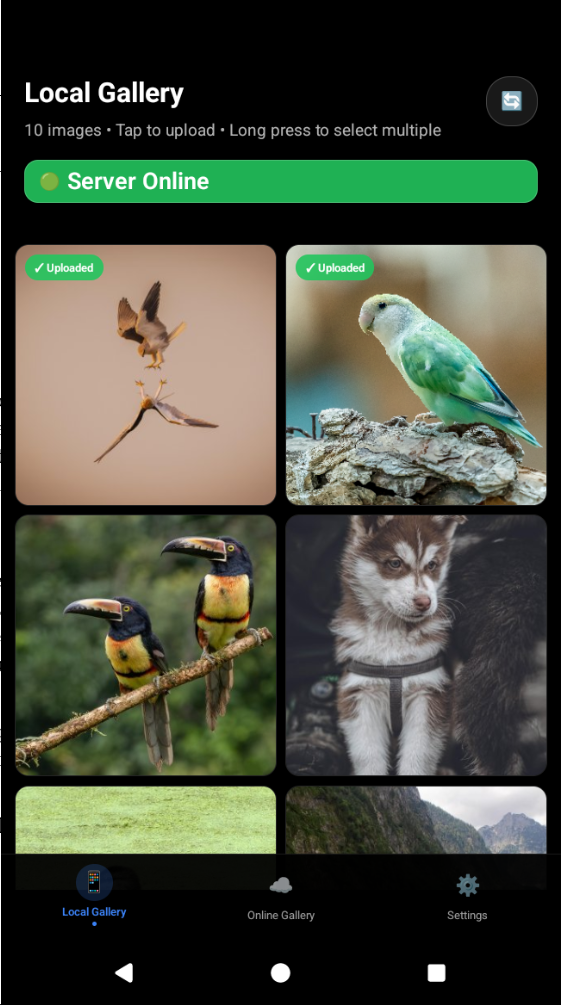
\includegraphics[width=\textwidth]{assets/local-gallery-mobile.png}
    \caption{Galería local en la aplicación móvil.}
    \label{fig:local-gallery-mobile}
  \end{minipage}
  \hfill
  \begin{minipage}[t]{0.3\textwidth}
    \centering
    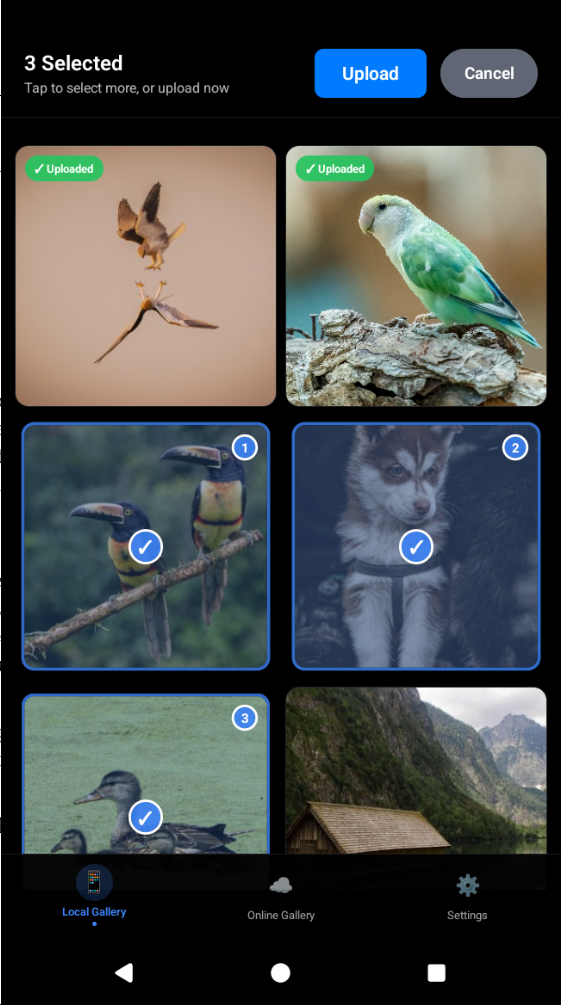
\includegraphics[width=\textwidth]{assets/local-gallery-selected-mobile.png}
    \caption{Galería local con varias imágenes seleccionadas.}
    \label{fig:local-gallery-selected-mobile}
  \end{minipage}
  \hfill
  \begin{minipage}[t]{0.3\textwidth}
    \centering
    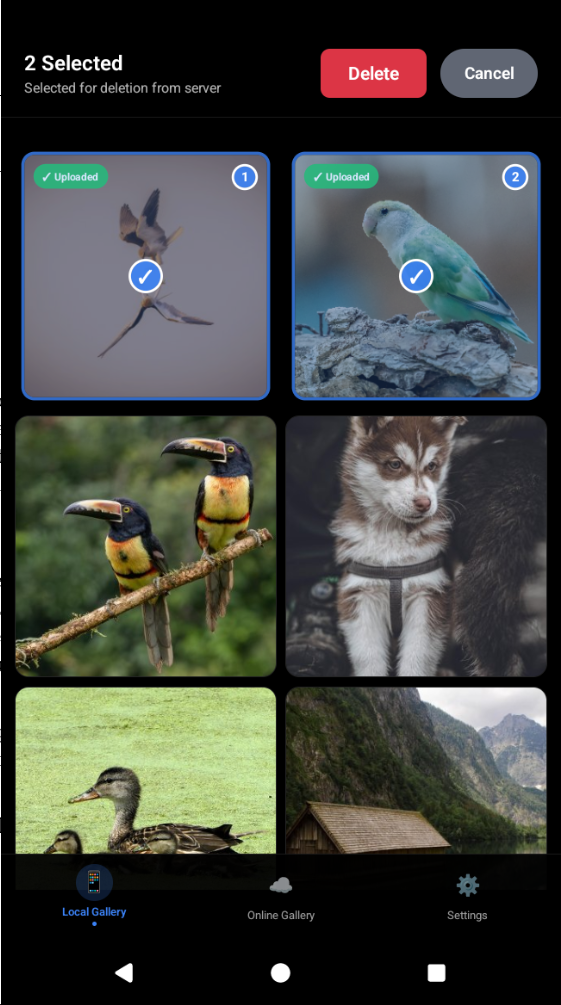
\includegraphics[width=\textwidth]{assets/local-gallery-delete-selected.png}
    \caption{Galería local con varias imágenes seleccionadas para eliminar del servidor.}
    \label{fig:local-gallery-delete-selected}
  \end{minipage}
\end{figure}

\section{Galería online}
Si navegamos a la galería online, podremos ver todas las imágenes que hemos subido al servidor desde cualquier dispositivo a nuestra cuenta. Desde esta galería, podremos eliminar las imágenes del servidor si lo deseamos o verlas en detalle.


\begin{figure}[H]
  \begin{minipage}[t]{0.3\textwidth}
    \centering
    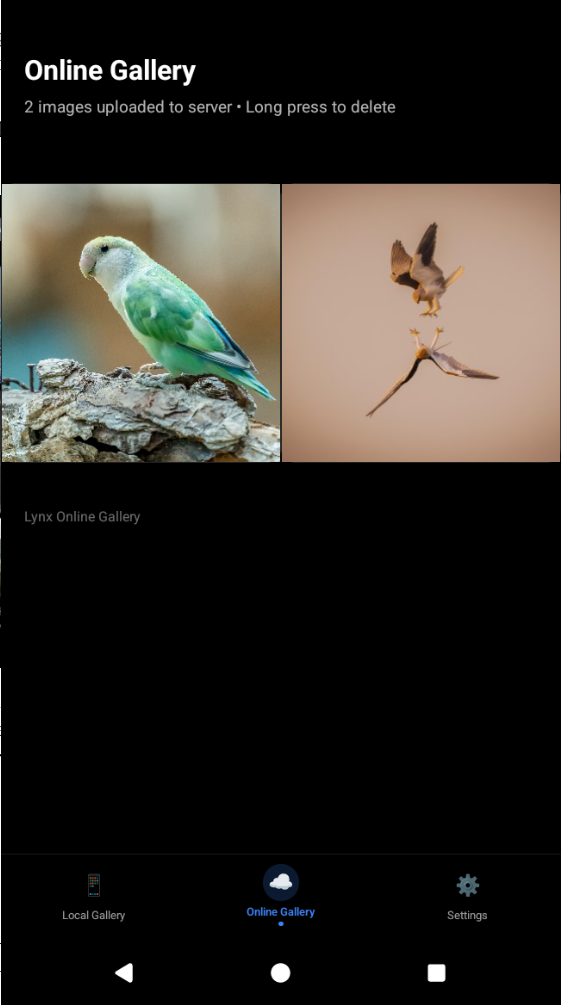
\includegraphics[width=\textwidth]{assets/online-gallery-mobile.png}
    \caption{Galería online en la aplicación móvil.}
    \label{fig:online-gallery-mobile1}
  \end{minipage}
  \hfill
  \begin{minipage}[t]{0.3\textwidth}
    \centering
    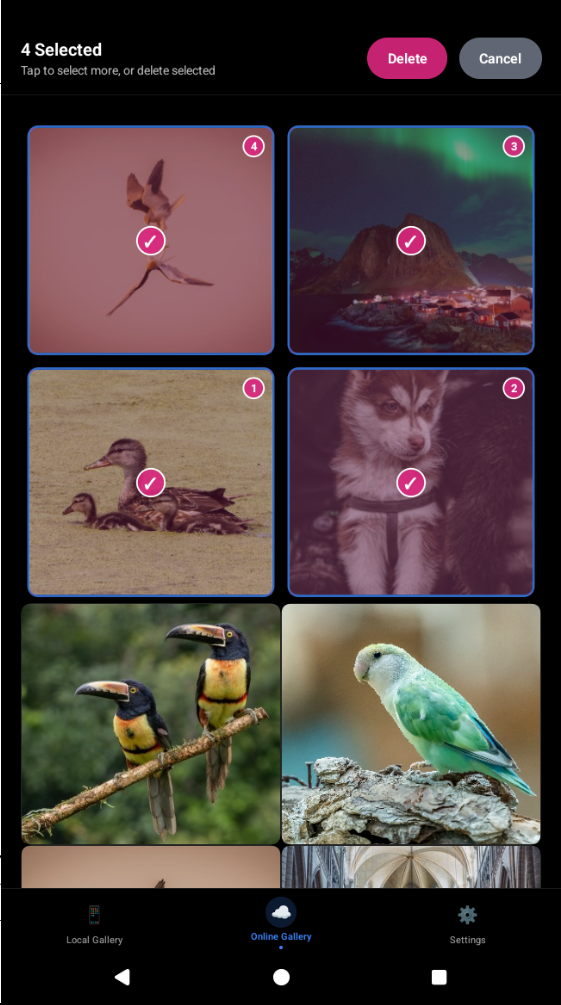
\includegraphics[width=\textwidth]{assets/online-gallery-mobile-2.png}
    \caption{Galería online seleccionando imágenes a borrar.}
    \label{fig:online-gallery-mobile1}
  \end{minipage}
\end{figure}

\section{Ajustes}
En el apartado de ajustes, podremos modificar los datos de conexión al servidor, activar o desactivar la sincronización automática, cambiar el número máximo de subidas concurrentes (para utilizar más o menos recursos del dispositivo móvil) y cerrar sesión. Los cambios solamente se aplicarán al pulsar el botón de guardar cambios. Una vez activada la opción de sincronización automática, entrar en la galería local hará que todas las imágenes que no hayan sido subidas al servidor se suban automáticamente.

\begin{figure}[H]
  \begin{minipage}[t]{0.3\textwidth}
    \centering
    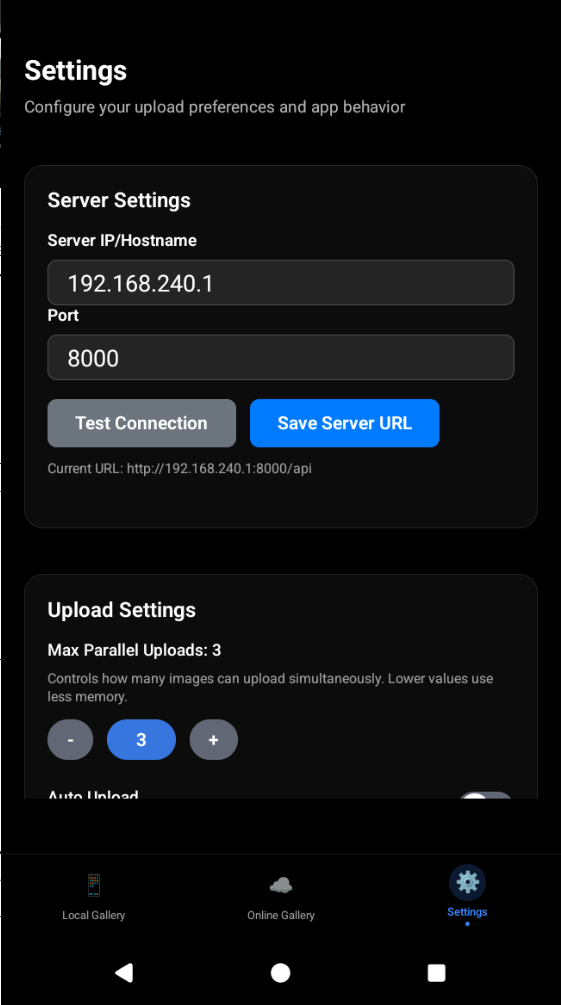
\includegraphics[width=\textwidth]{assets/settings-mobile1.png}
    \caption{Ajustes en la aplicación móvil. (1)}
    \label{fig:settings-mobile1}
  \end{minipage}
  \hfill
  \begin{minipage}[t]{0.3\textwidth}
    \centering
    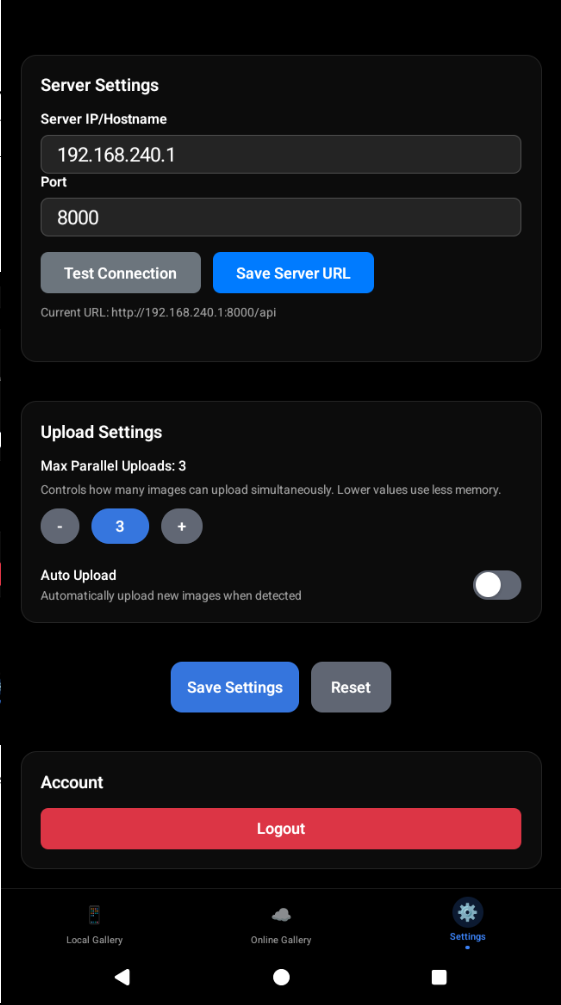
\includegraphics[width=\textwidth]{assets/settings-mobile2.png}
    \caption{Ajustes en la aplicación móvil. (2)}
    \label{fig:settings-mobile2}
  \end{minipage}
\end{figure}
